\chapter{Summary and Future Work} \label{c:summary}

This dissertation has described the motivation for, the design of, and the operation of a \SI{350}{\GHz} video imaging system intended for concealed weapons detection.
The system uses superconducting Transition Edge Sensor (\TES) bolometers to detect the \SI{350}{\GHz} light, and the first of four planned 251-detector sub-arrays has been installed into the system.
The spatial resolution is \SI{1.4}{\cm} FWHM at the system focus distance of \SI{17}{\m}, and the system has sufficient sensitivity to take video images that reveal the presence of a knife concealed under a cotton shirt.
At 6 frames per second, observing a $\SI{0.78}{\m} \times \SI{0.55}{\m}$ field of view with \SI{1}{\cm} pixels, the Noise Equivalent Temperature Difference (\NETD) of video frames observing a uniform temperature distribution is \SI{100}{\mK}.
This meets the requirements on \NETD\ outlined in \sectionref{sec:ch1-netd-reqs} for challenging passive imaging scenarios.
Video images of realistic scenes have higher \NETD\ due to artifacts of the scanning process, but algorithmic approaches to eliminating these artifacts have been outlined.

\section{Future Work on This System} \label{sec:ch8-future}

Future work on this system should focus on improving image processing algorithms, solving the existing technical problems and using the system to perform studies of passive imaging phenomenology.
Image processing was addressed in \sectionref{sec:ch7-algo}.

There are three technical problems with the system that should be addressed: the elliptical beams, the low optical efficiency, and the high detector noise.
It is not known whether the beam ellipticity is caused by a problem inside the cryostat (such as poor alignment between detectors and feedhorns) or outside the cryostat (such as poor alignment of the cryostat and beams with the primary and secondary mirrors).
One approach for distinguishing between these two possibilities is to measure the beam shapes immediately outside the cryostat window.
Manufacturing errors in one or more of the optical components are also a possibility.

Solving the optical efficiency problem requires understanding where in the optical chain the efficiency loss occurrs.
A first step towards understanding this would be to measure the optical efficiency at the cryostat window by chopping between warm and cold loads.
If this efficiency is higher that the efficiency at the far-field focal plane, this would be a sign that the lost efficiency is due to optical spillover.
If the efficiency is that same, this would indicate that the optical power is lost inside the cryostat.
Measurement of the far-field optical efficiency of all working detectors might reveal a trend across the focal plane, which could point to a fabrication problem with either the detetors or the feedhorn array.

Determining the source of the excess detector noise could be more challenging.
If the noise drops significantly when the cryostat is closed optically, that will be an indication that the problem is caused by excess photon noise.
Because the optical efficiency is poor, this photon noise would likely be caused by stray light reaching the detectors, so the \SI{1}{\K} focal plane should be checked carefully for this.
If high noise persists when the cryostat is optically closed, that could be a sign that the noise originates in the detectors, possibly due to dangling heat capacity.

A second 251-detector sub-array was fabricated simultaneously with the sub-array that is currently installed in the \Imager.
This sub-array was designed to have a $G$ value \SI{16}{\percent} lower than the sub-array that is currently installed, but should be otherwise identical.
If the detector noise, optical load, or optical efficiency are significantly different between these two sub-arrays, this could indicate a problem in fabrication.

% low g - 80 um legs
% hi g  - 67 um legs

Installation of the second sub-array will also improve system performance.
The additional detectors could be used to reduce image \NETD, increase the field of view, or increase the video frame rate.

Studies of phenomenology will focus on different sizes, shapes, and types of concealed objects, combined with different types of clothing.
Because the \Imager\ has been built by a team with little prior experience in the area of passive security imaging, we should identify partners among potential users of standoff passive imaging systems.
This will help us to ensure that the tests that we carry out will lead to results that are applicable to realistic operational scenarios, and can be compared to results using other imaging techniques.

\section{Polarization and Multi-band Imaging}

Following phenomenology studies using the existing system, there will be an opportunity to use it to test polarization-sensitive detectors as well as detectors that are sensitive to more than one optical band (i.e., multiple colors).
Polarization-sensitive and multi-color \TES\ detector technology already exists and could quickly be deployed into the existing system for testing.

Development of polarization-sensitive \TES\ bolometers has been driven by the desire to measure the polarization of the Cosmic Microwave Background radiation.
Polarization-sensitive focal planes have been installed in a number of telescopes and are currently taking data \cite{obrient_antenna-coupled_2012,austermann_sptpol:_2012,keating_ultra_2011,niemack_actpol:_2010,kusaka_modulation_2013}.
\figref{fig:ch8-multi-chroic} shows a photograph of a polarization-sensitive detector developed by a collaboration of which I am a member \cite{datta_horn_2014}.
Ring-loaded feedhorns direct light onto a pair of orthogonal ``fins'' which couple light onto microstrip transmission lines.
The light is then split into two frequency bands defined by quarter wave stub filters.
Each polarization in each frequency band is detected by a separate \TES\ bolometer. 
This allows a single feedhorn on the focal plane to detect not only two polarizations, but also two colors.

\begin{figure*}
\centering
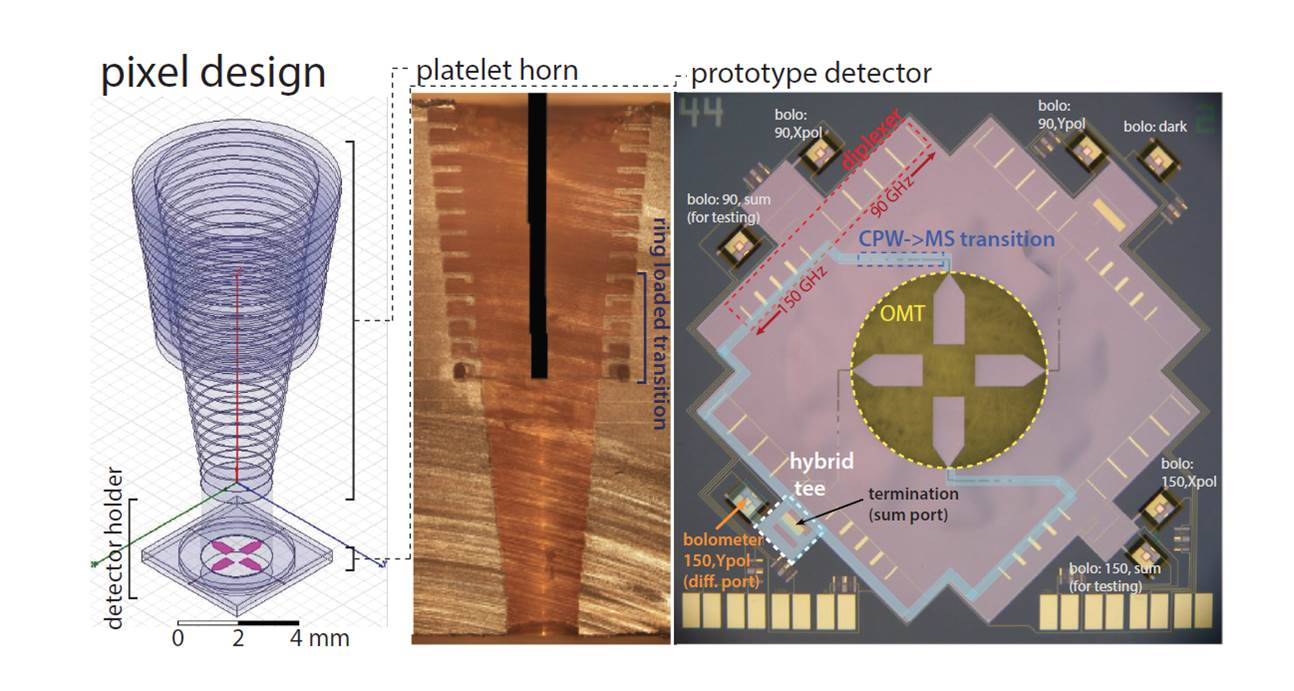
\includegraphics[width=\textwidth]{images/ch8-multi-chroic.jpg}
\caption[Multi-color, polarization-sensitive detectors]{
  A multi-color, polarization-sensitive detector.
  This detector is sensitive to both polarizations in bands centered at \SI{90}{\GHz} and \SI{150}{\GHz}.
  Light is coupled onto the detector by a ring-loaded feedhorn.
  On the left is a schematic of the feedhorns, in the middle is a cross-sectional photograph of a prototype feedhorn.
  The feedhorns are assembled from micro-machined silicon wafers that are then Au-plated.
  On the right is a prototype pixel.
  Two pairs of fins (``OMT'' couple each polarization onto microstrip.
  A diplexer separates the \SI{90}{\GHz} and \SI{150}{\GHz} signals.
  The ``hybrid tee'' rejects unwanted waveguide modes.
  This figure is taken from \cite{datta_horn_2014}, which contains more details on these detectors.
}
\label{fig:ch8-multi-chroic}
\end{figure*}

It is not clear whether polarization-sensitive detectors, or multi-color detectors, will provide advantages for passive security imaging.
Reflected light will be polarized to some extent, but since the concealed objects are illuminated from all directions, one would expect the net polarization to be low.
Nevertheless, there may be scenarios where uneven illumination is expected, and in such cases polarization may provide additional information.
Models addressing the usefulness of polarization for security imaging do exist, and should be used when deciding whether or not to build a polarization-sensitive system \cite{salmon_polarimetric_2004}.

The primary advantage of multi-color detectors is that they allow higher optical bandwidth while avoiding atmospheric absorption lines.
It may be that implementing band-stop filters could achieve the same benefit at lower cost.
An intriguing idea would be to attempt to use color information to identify different materials.
For example, many explosive materials have absorption features in the \SIrange{0.6}{3}{\THz} region \cite{federici_thz_2005,davies_terahertz_2008}.
Unfortunately most of these features are above \SI{1}{\THz}, where clothing and the atmosphere are much less transparent than at \SI{350}{\GHz}.

\section{Directions for Future Systems}

Following resolution of the remaining technical issues, and investigation of imaging phenomenology, we will be ready to design a second-generation system.
Such a system would be designed with a specific operational scenario in mind, which would set requirements for standoff distance, resolution and image \NETD.
But regardless of the details of the specifications, areas to focus on for such a system are likely to include size/portability and cost.

The overall system size is set by the standoff distance and desired spatial resolution, which directly determine the size of the optical aperture via \eqnref{eqn:ch1-raleigh}.
Moving to higher frequencies can reduce the size of the required optical aperture, but at the cost of lower image contrast due to decreased transmission through clothing and the atmosphere.
Nevertheless, this trade-off may be worthwhile for some applications.
There are no technical reasons why \TES\ bolometers could not work well at frequencies of \SI{1}{\THz}.

If the target application requires the aperture size to remain at \SI{1.3}{\m}, or even become larger, it may be desirable to use a different focusing element than that used in this system.
Possibilities include segmented mirrors (which have proven very successful for larger apertures \cite{fowler_optical_2007}) or a large-diameter Fresnel lens \cite{black_millimeter-wave_1987}.

Reducing the size of the optical aperture or moving to a Fresnel lens will likely reduce the cost of the system.
Three other ways to potentially reduce cost are to eliminate the need for scanning, operate at a higher bath temperature, or migrate to a detector technology that is easier to fabricate.

Eliminating the need for scanning will reduce cost by simplifying the design of the optical components and removing the need for motors to move those components.
But in order to maintain the same field of view, as well as ensure a Nyquist-sampled focal plane, many more detectors are required.
The cost and number of required detectors will depend on the desired field of view, optical design, and target wavelength.
Work on multiplexing techniques capable of reading out \num{10000} or more \TES\ detectors has begun \cite{irwin_advanced_2012}, but this technology is not as mature as the \TDM\ readout system used for the \Imager.
A careful cost analysis of all of these factors will need to be performed.

Operating at higher bath temperatures can reduce cost if the new bath temperature can be achieved without the use of a secondary cooling system such as the \He4-sorption refrigerator used for the \Imager.
As described in \sectionref{sec:det-parm-choice}, it should be possible to make photon-noise-limited \TES\ bolometers operating at a bath temperature of \SI{3.6}{\K}.
This bath temperature can be reached through the use of a cryocooler only, with no other refrigeration stages needed. 
The ideal $T_c$ for this bath temperature would be \abt{\SI{6.5}{\K}}.
TiNi films can easily be deposited ($T_c = \SI{5.6}{\K}$), or some other superconducting material could be used.
However, to-date little work has been done on making voltage-biased \TES\ bolometers work at such (relatively) high temperatures, so it is not clear what problems might appear that would need to be solved.
Again, a careful cost analysis is required.

Finally, voltage-biased \TES\ bolometers are not the only low-temperature detectors that can be fabricated in large quantities, read out with a reasonable number of wires, and achieve photon-noise-limited performance.
One very promising detector technology is the Microwave Kinetic Inductance Detector (\MKID).
As mentioned in \sectionref{sec:ch2-tes-passive}, one group is already working on a passive imaging system that will use these detectors.

Like \TES\ detectors, \MKIDs\ use superconducting materials at low temperatures, but the principle of operation is very different.
The superconducting material is chosen so that its gap energy is below the energy $h \nu$ of the photons to be detected.
Light is focused directly onto the superconducting film, so that it breaks Cooper pairs.
This induces a change in the inductance of the superconductor.
By making the superconductor a part of a resonant circuit, this change in inductance can be detected as a change in the resonant frequency of the circuit.
This approach to detection of light offers a natural way to multiplex many detectors on a single readout line, because the resonant frequency can be placed at \si{\GHz} frequencies where large amounts of readout bandwidth are available.

\MKID\ detectors reduce fabrication cost because fewer material layers and fabrication steps are required.
They also reduce wiring cost because a single coaxial cable can bias and read out many detectors.
But they also require more complicated room-temperature electronics to perform the readout, as well as low-noise amplifiers inside the cryostat.
The technology is also not yet as mature as \TES\ detectors with multiplexed SQUID readout.
Once again, a careful evaluation of the costs and benefits of \MKID\ detectors will need to be performed.

In summary, several promising approaches for reducing system portability, cost, and complexity are available.
The \Imager\ described in this dissertation demonstrates that \SI{100}{\mK} \NETD\ video images at \SI{17}{\m} standoff distances are achievable using large-format arrays of cryogenic detectors.
Following resolution of the remaining technical issues and investigation of imaging phenomenology, we will be ready to design a second-generation system.
The second-generation system will start to bring the advantages of practical, cost-effective, high-sensitivity passive imaging to the security community.
